\setlength{\multlinegap}{0pt}
\section{Theorie}
\subsection{$\beta$-Zerfall}
Der $\beta$-Zerfall liefert im Gegensatz zum $\alpha$- und $\gamma$-Zerfall ein kontinuierliches Energiespektrum. Das warf Fragen auf, denn als Zerfallsprodukt konnte nur ein Elektron, bzw. ein Positron, detektiert werden. Dies erfüllte aber weder Energie- noch Impuls- und Drehimpulserhaltung. Abhilfe schaffte 1931 Wolfgang Pauli, indem er ein weiteres Teilchen postulierte, das Neutrino. Da dies einen halbzahligen Spin besitzt, war damit der Drehimpuls erhalten. Außerdem trägt es den fehlenden Teil der Energie und des Impulses. Außerdem trägt auch das Nukleon einen Teil des Impulses als Rückstoß. Dargestellt ist diese Impulsverteilung in \cref{beta}.

%\begin{figure}[h]
%	\centering
%	\imcludegraphics[width=0.9\textwidth]{betazerfall.png}
%	\label{beta}
%	\caption{Impulsverteilung beim $\beta^-$-Zerfall mit $p_e$ dem Impuls des Elektrons, $p_\nu$ dem Impuls des Antineutrinos und $p_r$ dem Impuls des Rückstoßes.}
%\end{figure}

Es gibt drei verschiedene Arten des $\beta$-Zerfalls, die aber alle gemein haben, dass ein Nukleon umgewandelt wird. Beim $\beta^-$-Zerfall (\cref{eq:beta-}) wird ein Neutron zu einem Proton und erzeugt dabei außerdem ein Elektron und ein Elektron-Antineutrino. Beim $\beta^+$-Zerfall (\cref{eq:beta+}) wird ein Proton zu einem Neutron unter Erzeugung eines Positrons und eines Elektron-Neutrinos. Der dritte Prozess ist der Elektroneneinfang, auch electron capture genannt (\cref{eq:ec}). Hierbei muss sich ein Elektron sehr nah am Atomkern befinden, sodass es mit einem Proton zu einem Neutron und einem Elektron-Neutrino reagieren kann.

\begin{align}
	\beta^-&:	 n \rightarrow p + e^- + \overline{\nu_e} \label{eq:beta-} \\
	\beta^+&:	 p \rightarrow n + e^+ + \nu_e \label{eq:beta+} \\
	\text{ec}&: p + e^- \rightarrow n + \nu_e \label{eq:ec}
\end{align}

Da die Masse des Protons geringfügig kleiner ist als die des Neutrons, können sowohl $\beta^-$-Zerfalls als auch electron capture nicht an freien Protonen stattfinden, sondern nur im Atomkern. Der $\beta^+$-Zerfalls dagegen ist auch an freien Neutronen möglich.

\section{Tröpfchenmodell}
Ob bei einem Kern ein $\beta$-Zerfall auftritt, hängt von der Energie und damit von der Masse des Kerns ab. Diese ist durch die Weizsäckersche Masseformel in \cref{eq:masse} beschrieben, mit $m_p$ der Masse eines Protons, $m_n$ der Masse eines Neutrons und $B$ der Bindungsenergie.

\begin{equation}
	m(A,Z) = Zm_p + (A-Z)mn-B
	\label{eq:masse}
\end{equation}

Besonders interessant ist hier die Bindungsenergie. Sie wird durch das Tröpfchenmodell mithilfe der halbempirischen Bethe-Weizsäcker-Formel (siehe unten) bestimmt.

\begin{align*}
	&a_V A  &&:\text{Volumenterm}\\
	-&a_S A^{2/3} &&:\text{Oberflächenterm}\\
	-&a_C Z^2 A^{2/3} &&:\text{Coulombterm}\\
	-&a_A \frac{(Z-N)^2}{4A} &&:\text{Asymetrieterm}\\
	+&\begin{cases}
		+\delta  &\text{für gg-Kerne}\\
		0 &\text{für ug- oder gu-Kerne} \\
		-\delta &\text{für uu-Kerne} 
	\end{cases}&&:\text{Paarterm}
\end{align*}

Dabei wird der Atomkern ähnlich wie ein Wassertropfen betrachtet. Die Formel setzt sich aus fünf Termen zusammen:

\begin{itemize}
\item Der erste und größte Term ist der Volumenterm. Er ist proportional zum Radius des Kerns und beschreibt die "Kondensationsenergie" der Nukleonen. Aufgrund des Zusammenhangs $A^{1/3} \propto r_\text{Kern}$, und da der Kern auf alle drei Raumdimensionen ausgedehnt ist, ist der Volumenterm linear von der Nukleonenzahl abhängig.

\item Da die Nukleonen an der Oberfläche nur nicht so viele Bindungspartner haben wie die Nukleonen im Inneren des Kerns, verringert der Oberflächenterm die Bindungsenergie proportional zur Oberfläche des Kerns.

\item Der Coulombterm berücksichtigt die positive Ladung der Protonen, die sich abstoßen. Daraus ergibt sich mit der Formel für die Coulomb-Energie einer geladenen Kugel $E \propto q^2/r = Z^2/A^{1/3}$

\item Die Protonen und Neutronen sortieren sich im Kern unabhängig voneinander auf Energieniveaus, jeweils zwei Teilchen pro Niveau. Wenn also deutlich mehr Teilchen der einen Sorte im Kern vorhanden sind, müssen sich diese auf deutlich höheren Energieniveaus befinden als bei einer gleichen Verteilung zwischen Protonen und Neutronen. Dieser Umstand wird durch den Asymetrieterm in der Formel berücksichtigt.

\item Da auf jedes Energieniveau jeweils zwei Teilchen passen, muss für ein weiteres Teilchen ein neues höheres Energieniveau besetzt werden. Daher haben Kerne, die aus einer geraden Anzahl an Protonen und Neutronen bestehen, eine höhere Bindungsenergie und sind somit energetisch günstiger als Kerne mit ungerader Anzahl an Protonen und Neutronen.
\end{itemize}

\section{Methoden}
Um ein $\beta$-Spektrum messen zu können werden die erzeugten Elektronen in einem Magnetfeld abgelenkt. Die Bahnkurve wird dabei durch Lorentz- und Zentripetalkraft gegeben. Im homogenen Magnetfeld ergibt sich mit $m$ der relativistische Masse so:

\begin{equation}
Bev = \frac{mv^2}{\rho}.
\label{bfeld}
\end{equation}

Die Teilchen beschreiben dabei eine kreisförmige Bahnkurve. Da der Impuls durch $p = eB\rho$ gegeben ist, sortiert das Spektrometer die Teilchen nach Impuls. Für die Messung mit dem Spektrometer sind zwei Größen wichtig: Die Impulsauflösung und die Transmission. Die Transmission ist ein Maß dafür, wie viele der von der Quelle emittierten Elektronen vom Detektor detektiert werden. Sie wird über

\begin{equation}
T = N(Det)/N(4\pi)
\label{eq:transmission}
\end{equation}

bestimmt. Sie steigt, je größer der Eintrittsspalt des Detektors ist. Die Impulsauflösung wird über die relative Linienbreite bestimmt. Diese ist konstant und wird auch Apparaturkonstante genannt. Sie wird mithilfe der Formel

\begin{equation}
R = \frac{\Delta p}{p} = \frac{\Delta(B\rho)}{B\rho} = \frac{\Delta\rho}{\rho}
\label{eq:apparaturkonstante}
\end{equation}

berechnet. Die Impulsauflösung beträgt meist etwa $1\%$. Sie verschlechtert sich bei größerem Eintrittsspalt und verbessert sich bei kleinerem Eintrittsspalt. Die beiden Größen können also nicht gleichzeitig optimiert werden. Außerdem werden bei einem Spektrometer, dass die Elektronen nur in einer Ebene ablenkt, alle Elektronen nicht berücksichtigt, die nicht in dieser Ebene emittiert werden. Ein Spektrometer, der für diese Probleme eine Lösung anbietet, ist das im Versuch verwendete Toroid-Spektrometer. Der Aufbau dieses Spektrometers ist in \cref{skizze} dargestellt.

%\begin{figure}[h]
%	\centering
%	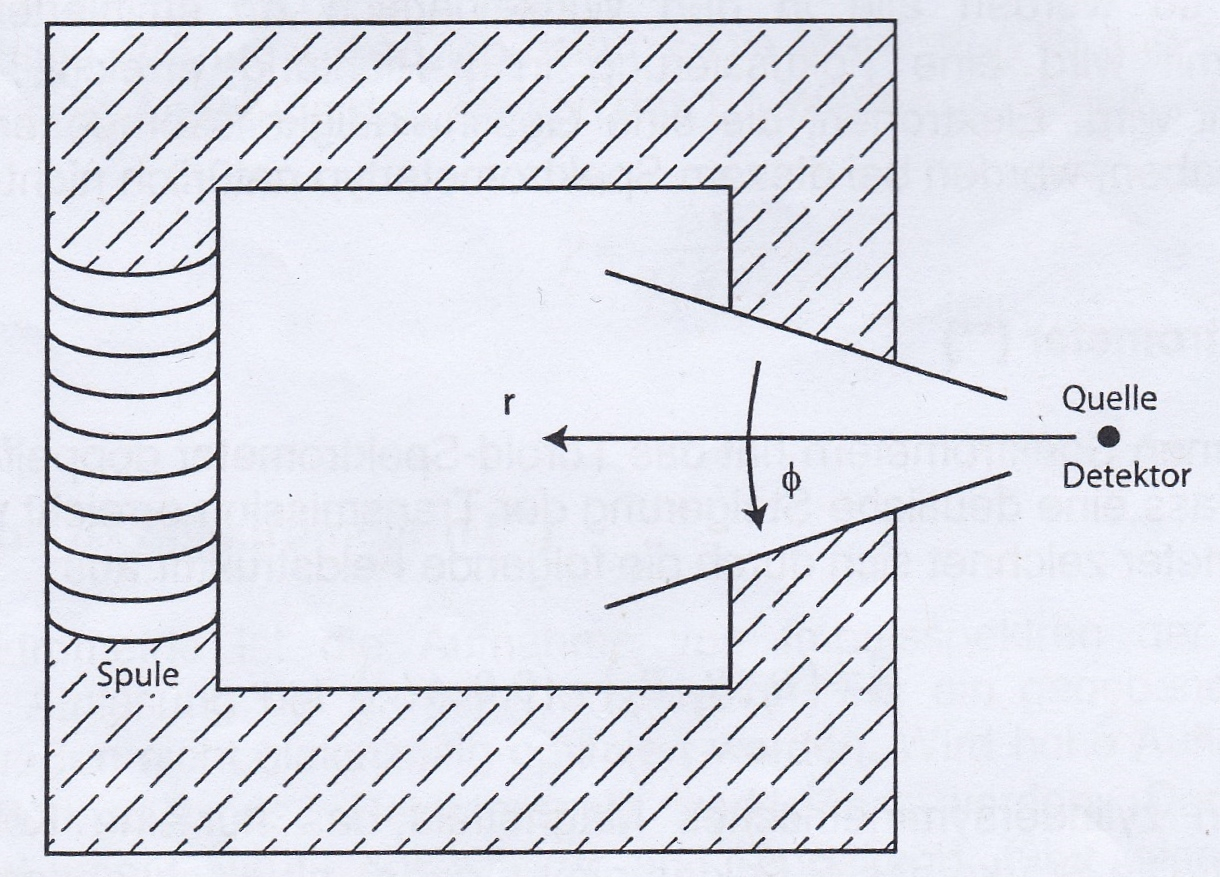
\includegraphics[width=0.9\textwidth]{Skizze.png}
%	\label{skizze}
%	\caption{Schematischer Aufbau des Toroid-Spektrometers}
%\end{figure}

Dabei liegen Quelle und Detektor in dieser Graphik genau hintereinander, der Detektor ist allerdings um $2\rho$ nach hinten verschoben. Die Elektronen werden von der Quelle emittiert und gelangen dann in das Magnetfeld, das von den Polschuhplatten erzeugt wird. Die Lorentzkraft lenkt die Elektronen dann auf den Detektor, wo diese gemessen werden können. Die Öffnungen, an denen Quelle und Detektor liegen, sind keilförmig. Das Magnetfeld, von dem die Elektronen abgelenkt werden, ist zylindersymmetrisch und besitzt nur eine Komponente in $\Phi$-Richtung. In \cref{feldlinien} ist das B-Feld als Draufsicht auf die r-$\Phi$-Ebene gezeigt. Erkennbar ist, dass die Feldstärke bei größerem r abnimmt. Dies sorgt für die trochoide Bahn, die die Elektronen beschreiten. 

%\begin{figure}[h]
%	\centering
%	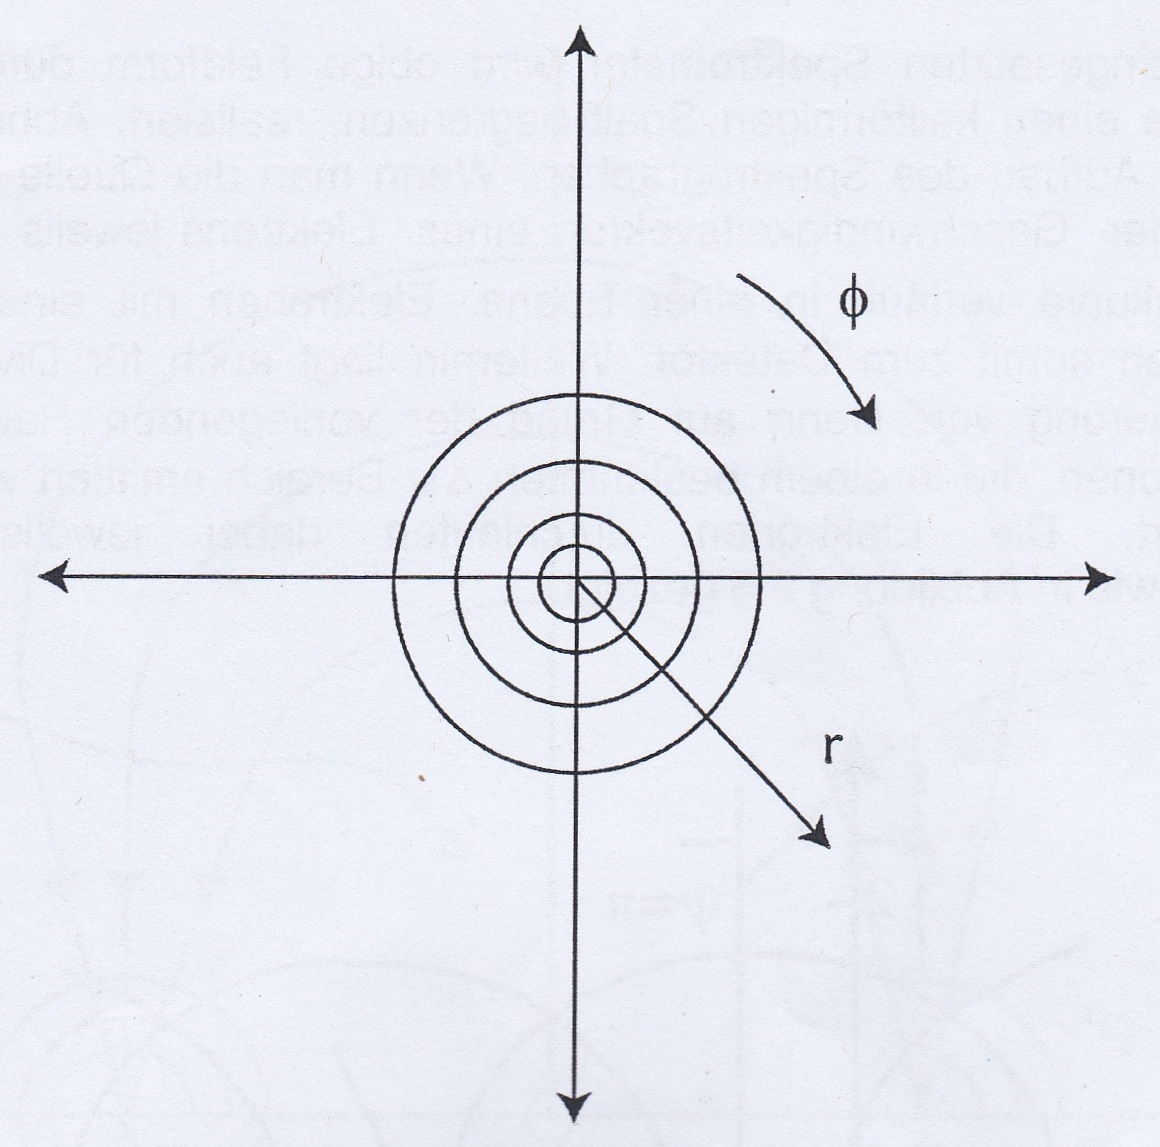
\includegraphics[width=0.9\textwidth]{Feldlinien.png}
%	\caption{Das B-Feld des Spektrometers als Draufsicht auf die r-$\Phi$-Ebene}
%	\label{feldlinien}
%\end{figure}

Dadurch können nicht nur Elektronen aus einer Ebene detektiert werden, sondern auch solche, die in andere Raumrichtungen emittiert wurden. Das wird in \cref{ebahn} deutlich. Hier sind die Trochoiden deutlich erkennbar. Dies verbessert die Transmission deutlich, während die Auflösung gleich bleibt.

%\begin{figure}[h]
%	\centering
%	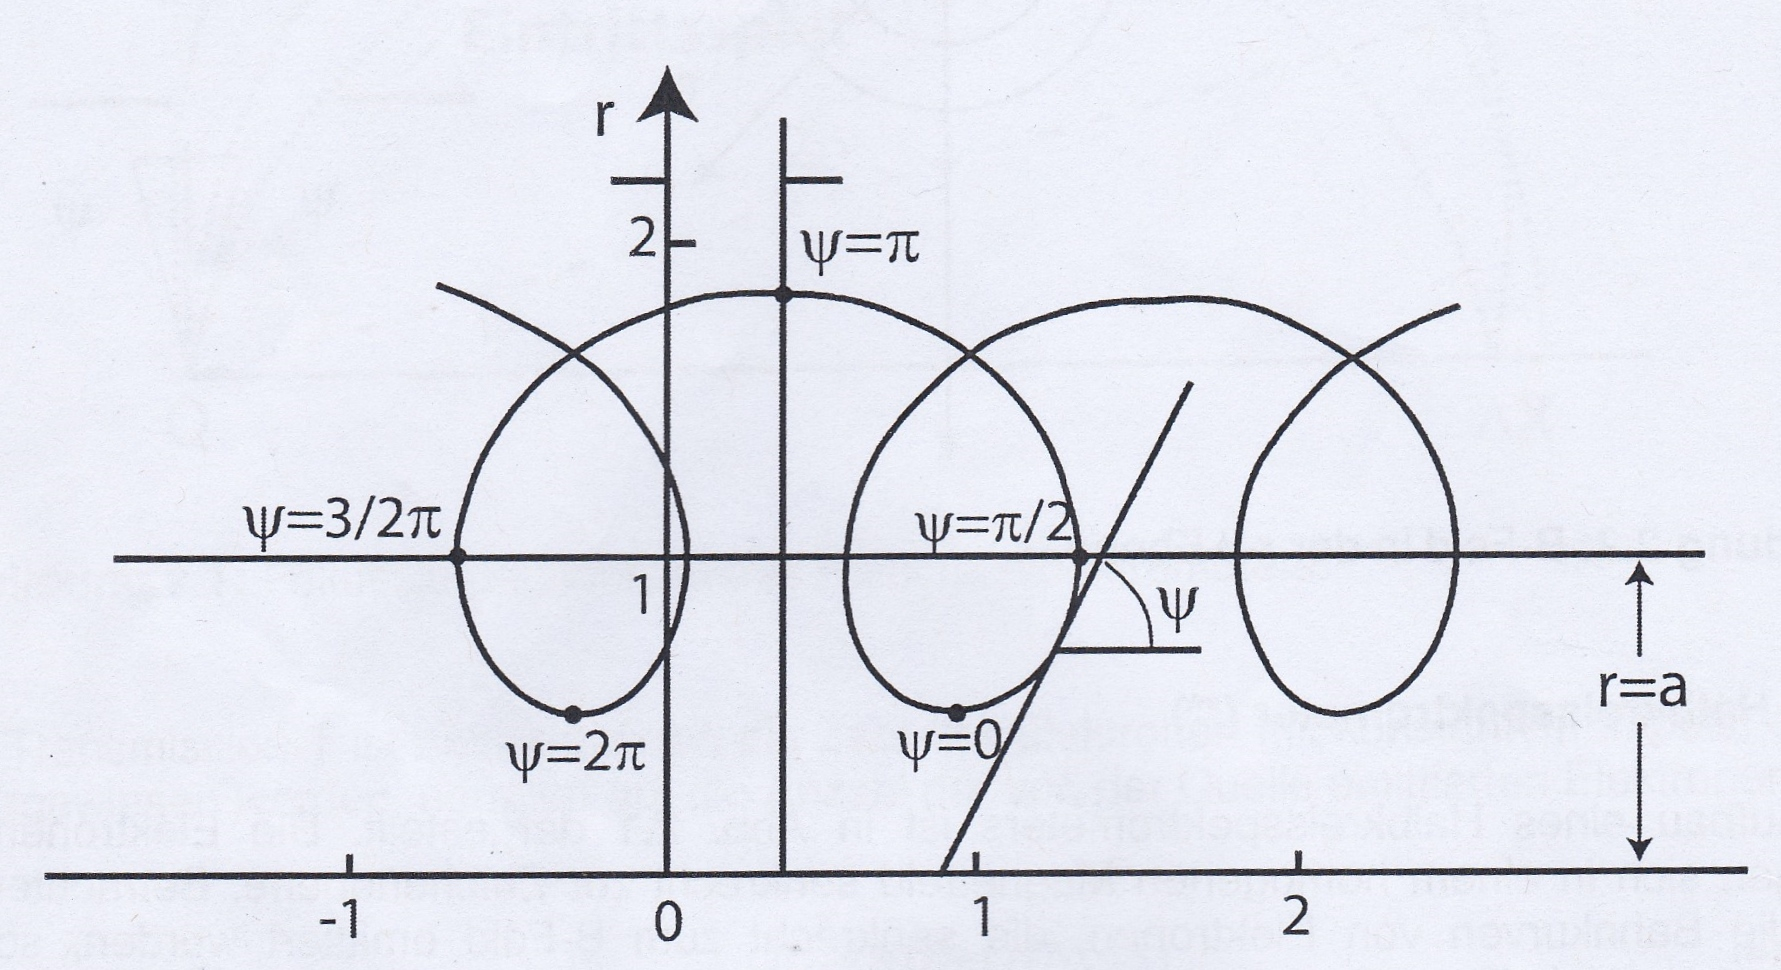
\includegraphics[width=0.9\textwidth]{Elektronenbahn.png}
%	\label{ebahn}
%	\caption{Elekronenbahn im toroidalen Feld der Polschuhplatten. Man erkennt die Fokussierung, die dafür sorgt, dass auch Elektronen, die nicht in der Ebene von Quelle und Detektor emittiert wurden, auf den Detektor geschickt werden.}
%\end{figure}

Vom Detektor laufen sie gemäß \cref{aufbau} durch einige weitere Bauteile, bevor das Signal zur Auswertung bereit ist.

%\begin{figure}[h]
%	\centering
%	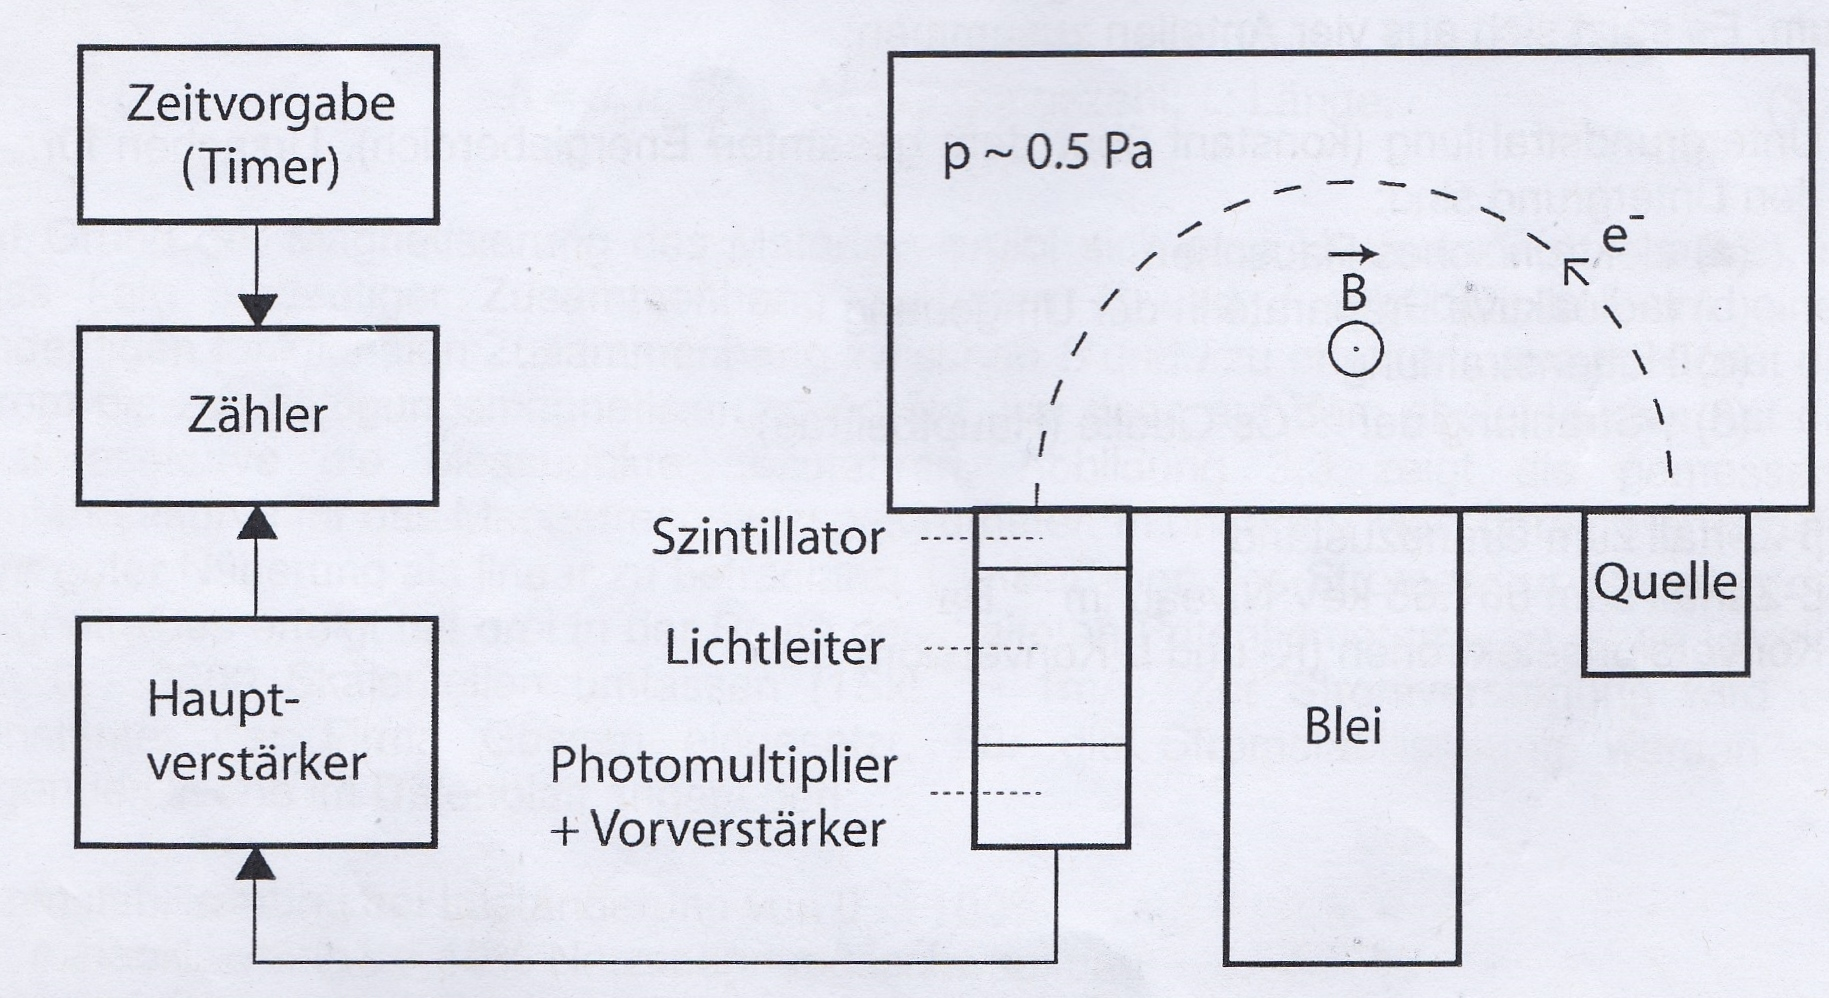
\includegraphics[width=0.9\textwidth]{Aufbau.png}
%	\label{aufbau}
%	\caption{Schematische Darstellung des Versuchaufbaus.}
%\end{figure}

Zuerst wird das Elektron von einem Szintillator detektiert. Von dort wird es in einem Photomultiplier verstärkt. Dabei wird das Elektron auf eine Dynode beschleunigt, aus der es aufgrund der hohen kinetischen Energie mehrere Elektronen lösen kann. Diese werden nun auf weitere Dynoden gelenkt, sodass am Ende viele Elektronen zum Signal beitragen. Dieses wird am Vorverstärker weiter verstärkt, bevor es am Hauptverstärker in einen Rechteckpuls umgewandelt wird. Dieser erreicht schließlich den Zähler. Zur weiteren Verarbeitung wird ein selbsterstelltes Programm in der graphischen Programmiersprache LabView verwendet.